\documentclass{beamer}
\usepackage{polski}
\usepackage[utf8]{inputenc}
\usepackage{graphicx}
\usetheme{AGH}
\author{Marcin Fabrykowski}
\title{Analiza i przetwarzanie obrazu\\Filtry nieliniowe}
\begin{document}
\begin{frame}
\maketitle
\end{frame}
\begin{frame}
\frametitle{O czym będziemy mówić}
\tableofcontents
\end{frame}
\section{Filtry logiczne}
\begin{frame}
\frametitle{Filtry logiczne}
\begin{block}{zasada działania}
\only<1->{wartość pixel określana jest na podstawie zależności sąsiadów}
\only<2->{
	\begin{tabular}{|c|c|c|}
	\hline
	&a&\\
	\hline
	b&X&c\\
	\hline
	&d&\\
	\hline
	\end{tabular}
	}
\end{block}
\begin{block}{zastosowanie}<3->
\begin{itemize}
\item Usuwanie poziomych lini:\\p = a, jeśli a=d, w~przeciwnym przypadku X
\item Usuwanie pojedynczych punktów:\\p = a, jeśli a=b=c=d, w~przeciwnym przypadku X
\end{itemize}
\end{block}
\end{frame}

\section{Filtr medianowy}
\begin{frame}
\frametitle{Filtr medianowy}
\begin{block}{Zastosowanie}<1->
usuwanie szumów z obrazu
\end{block}
\begin{block}{Zasada działania}<2->
wybierany jest element środkowy z okna
\end{block}
\begin{block}{Popularne okna}<3->
3x3, 5x5, 7x7
\end{block}
\end{frame}
\begin{frame}
\only<1>{\frametitle{Przykładowe działanie: okno 3x3}
}
\only<2>{\frametitle{Przykładowe działanie: okno 7x7}
\addtocounter{framenumber}{1}
}
\only<3>{\frametitle{Przykładowe działanie: okno 13x13}
\addtocounter{framenumber}{1}
}
\begin{figure}
\hspace{-200px}
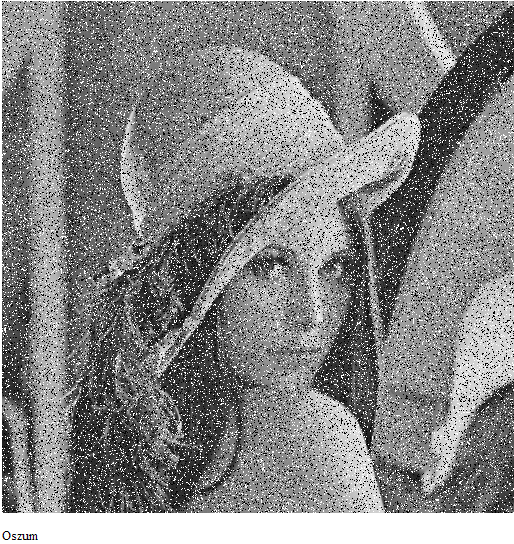
\includegraphics[width=150px]{medianowy_szum}
\end{figure}
\begin{figure}
\only<1>{
\vspace{-183px}
\hspace{150px}
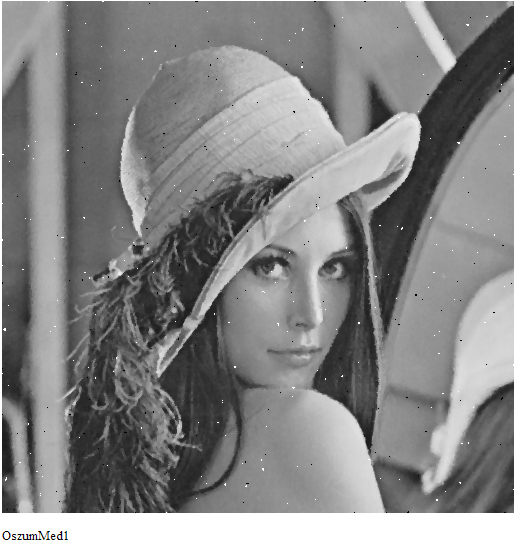
\includegraphics[width=150px]{medianowy_3x3}
}
\only<2>{
\vspace{-183px}
\hspace{150px}
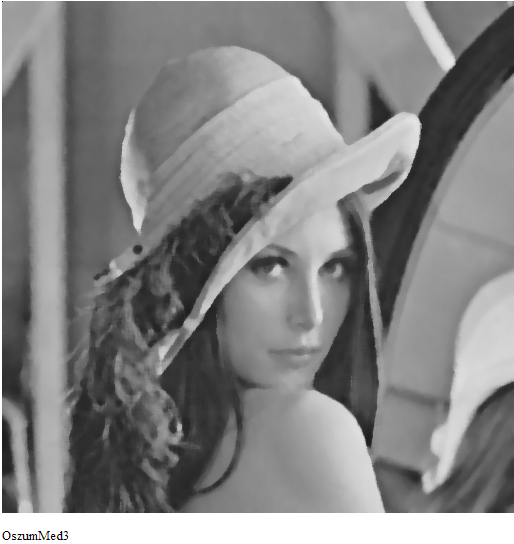
\includegraphics[width=150px]{medianowy_7x7}
}
\only<3>{
\vspace{-183px}
\hspace{150px}
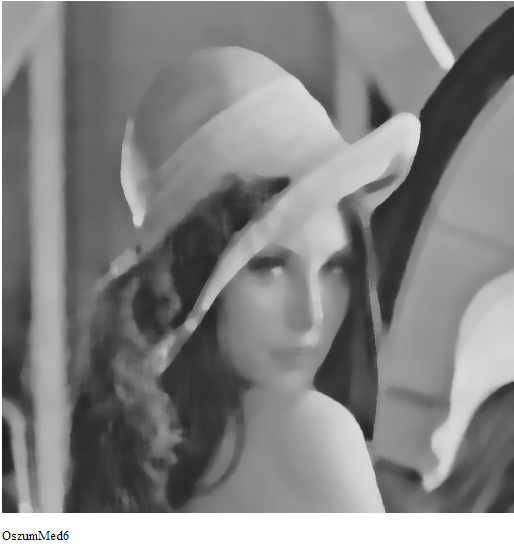
\includegraphics[width=150px]{medianowy_13x13}
}
\end{figure}
\end{frame}
\begin{frame}
\frametitle{Wady i zalety rozmiarów okien}
\begin{block}{Mniejsze okna}<1->
\begin{itemize}
\item krótszy czas filtrowania
\item wyraźniejszy obraz
\item obecność niepożądanych efektów
\end{itemize}
\end{block}
\begin{block}{Większe okna}<2->
\begin{itemize}
\item dłuższy czas filtrowania
\item niewyraźny obraz
\item brak niepożądanych efektów
\end{itemize}
\end{block}
\end{frame}
\begin{frame}
\frametitle{Czy można lepiej?}
\begin{figure}
\hspace{-200px}
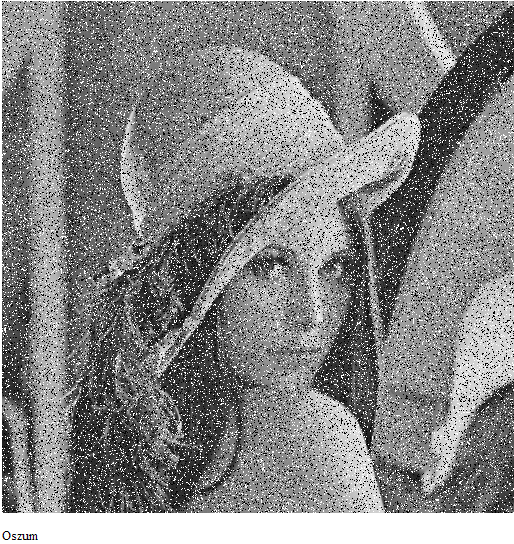
\includegraphics[width=150px]{medianowy_szum}
\end{figure}
\begin{figure}
\only<1>{
\vspace{-183px}
\hspace{150px}
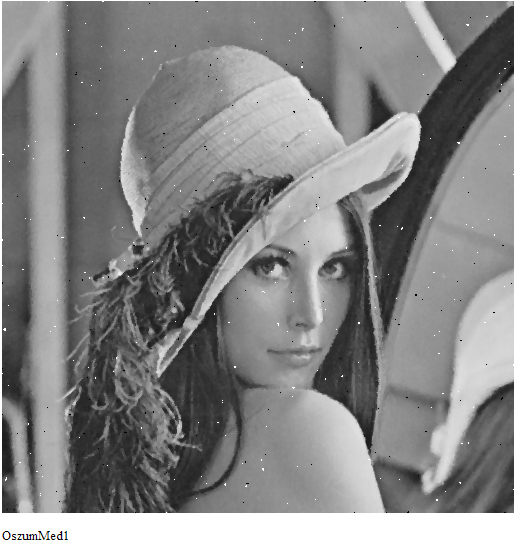
\includegraphics[width=150px]{medianowy_3x3}
}
\only<2>{
\addtocounter{framenumber}{1}
\vspace{-183px}
\hspace{150px}
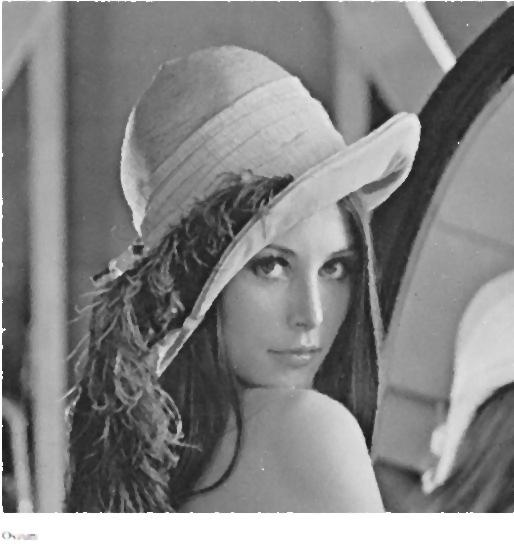
\includegraphics[width=150px]{medianowy_3x3_2}
}
\end{figure}
\end{frame}
\begin{frame}
\frametitle{Filtr medianowy vs uśredniający}
\begin{figure}
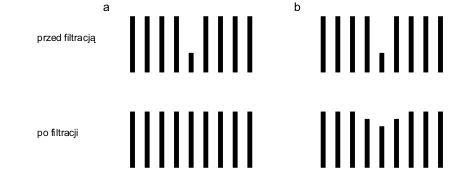
\includegraphics[height=80px]{median_vs_avg2}
\end{figure}
\begin{figure}
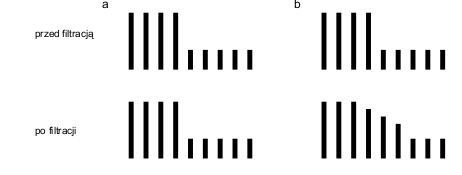
\includegraphics[height=80px]{median_vs_avg3}
\end{figure}
\end{frame}
\begin{frame}
\frametitle{Filtr medianowy vs uśredniający}
\begin{figure}
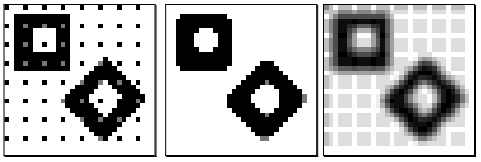
\includegraphics[height=80px]{median_vs_avg1}
\end{figure}
\end{frame}
\section{Filtry minimalny i maksymalny}
\begin{frame}
\frametitle{Filtry minimalny i maksymalne}
\begin{block}{zasada działania}
działają podobnie jak filtr medianowy, z tą różnicą że wybierany jest odpowiednio najmniejszy bądź największy element
\end{block}
\begin{block}{zastosowanie}
Minimalny(erozja) powoduje zmniejszanie się elementów obrazu, natomiast maksymalny(dylatacja) powoduje ich zwiększanie
\end{block}
\end{frame}
\begin{frame}
\frametitle{Erozja i dylatacja}
\begin{figure}
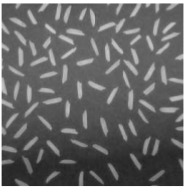
\includegraphics[width=100px]{min_max_min}
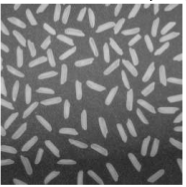
\includegraphics[width=100px]{min_max_orig}
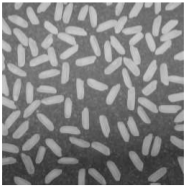
\includegraphics[width=100px]{min_max_max}
\end{figure}
\end{frame}


\section{Wykrywanie krawędzi}
\begin{frame}
\frametitle{Kombinowane wykrywanie krawędzi}
\begin{block}{Zasada działania}
stosujemy filtry poziomy i pionowy, a następnie obliczamy odległości euklidesowe dla odpowiednich punktów:\\
$p = \sqrt{p_h^2 + p_v^2}$
\end{block}
\begin{block}{uproszczenie}
dla uproszczenia obliczeń, stosuje się czasem sumę modułów:\\
$p = |p_h| + |p_v|$
\end{block}
\end{frame}
\begin{frame}
\frametitle{Wykrywanie krawędzi}
\begin{figure}
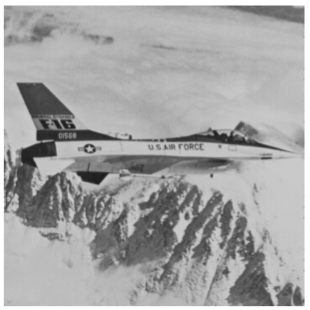
\includegraphics[height=150px]{krawedzie_orig}
\end{figure}
\end{frame}
\begin{frame}
\frametitle{Wykrywanie krawędzi}
\begin{figure}
\hspace{-200px}
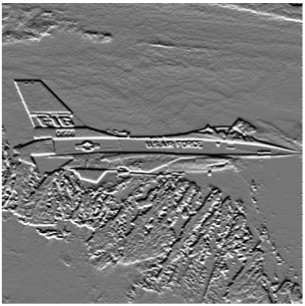
\includegraphics[width=150px]{krawedzie_poziome}
\end{figure}
\begin{figure}
\only<1>{
\vspace{-176px}
\hspace{150px}
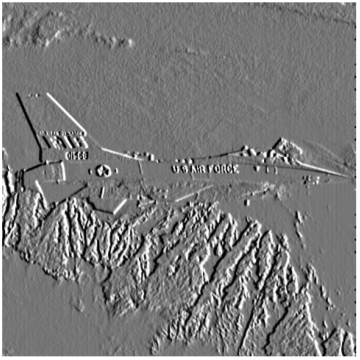
\includegraphics[width=150px]{krawedzie_pionowe}
}
\end{figure}
\end{frame}
\begin{frame}
\frametitle{Wykrywanie krawędzi}
\begin{figure}
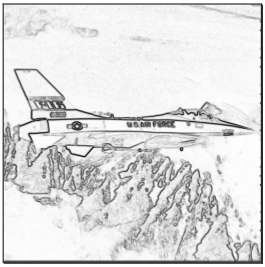
\includegraphics[width=150px]{krawedzie_kombinowane}
\end{figure}
\end{frame}
\section{Filtry adaptacyjne}
\begin{frame}
\frametitle{Filtry adaptacyjne}
\begin{block}{zastosowanie}<1->
wykorzystywane w celu podniesienia skuteczności innych filtrów
\end{block}
\begin{block}{przykłady}<2->
adaptacyjny uśredniający, adaptacyjny medianowy
\end{block}
\end{frame}
\begin{frame}
\frametitle{Podsumowanie}
\begin{block}{Wady}<1->
\begin{itemize}
\item trudniejsze w implementacji
\item dłuższy czas wykonywania
\end{itemize}
\end{block}
\begin{block}{Zalety}<2->
\begin{itemize}
\item znacznie lepsze efekty działania
\end{itemize}
\end{block}
\end{frame}
\begin{frame}
\frametitle{Ostateczna konfrontacja}
\begin{figure}
\only<1>{
	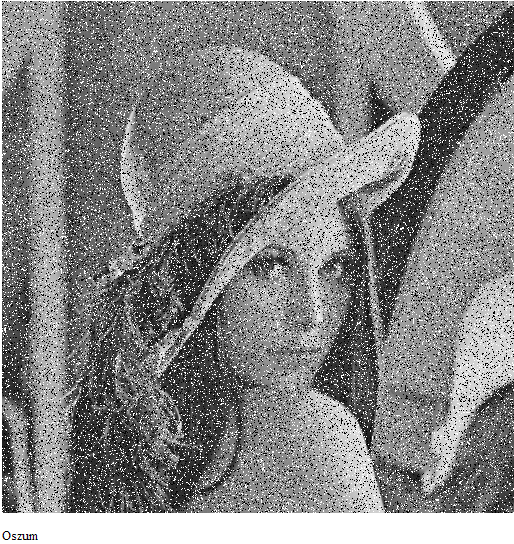
\includegraphics[width=150px]{medianowy_szum}
}
\only<2>{
	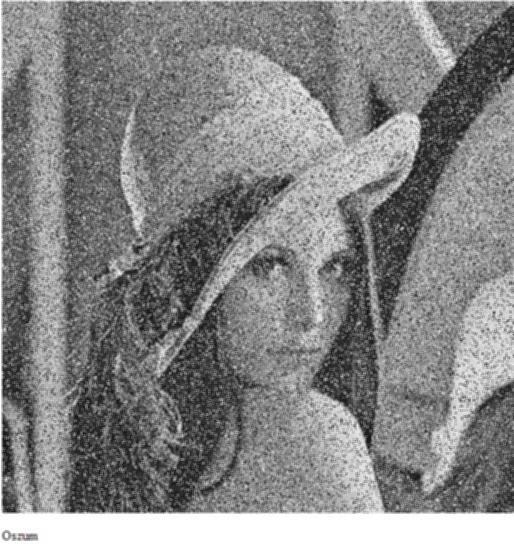
\includegraphics[width=150px]{usredniajacy}
	\addtocounter{framenumber}{1}
}
\only<3>{
	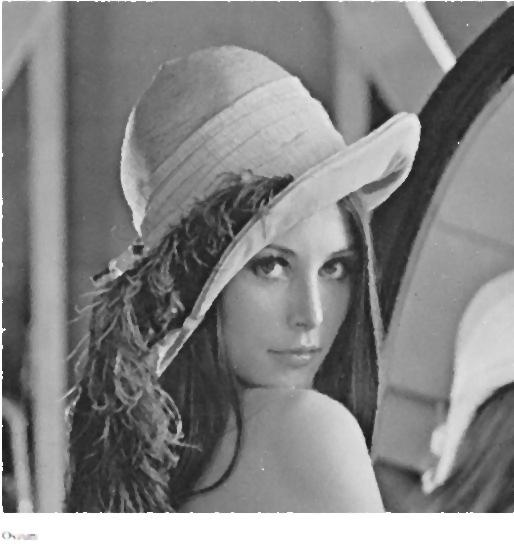
\includegraphics[width=150px]{medianowy_3x3_2}
	\addtocounter{framenumber}{1}
}
\end{figure}
\end{frame}
\begin{frame}
\frametitle{Bibliografia}
\footnotesize{
\bibliographystyle{plain}
\bibliography{FabrykowskiMarcin}}
\nocite{*}
\normalsize
\end{frame}
\end{document}
